\documentclass{article}


\usepackage{arxiv}
\usepackage{graphicx}
\usepackage{amsmath}

\usepackage[utf8]{inputenc} % allow utf-8 input
\usepackage[T1]{fontenc}    % use 8-bit T1 fonts
\usepackage{hyperref}       % hyperlinks
\usepackage{url}            % simple URL typesetting
\usepackage{booktabs}       % professional-quality tables
\usepackage{amsfonts}       % blackboard math symbols
\usepackage{nicefrac}       % compact symbols for 1/2, etc.
\usepackage{microtype}      % microtypography
\usepackage{lipsum}

\title{BBM-497 Assignment 1}


\author{
  Hakan AKYÜREK \\
  \texttt{b21426553@cs.hacettepe.edu.tr} \\
  %% examples of more authors
}

\begin{document}
\maketitle

\section{Introduction}
In this report I discuss my approaches to given tasks, namely author detection and essay generation, my approach to language model structure, and analysis of results.
\section{Language Model}

I used a Bag of Words(BoW) model for the tasks. I have trained 3 for each author, 6 in total, models, which are all able to both generate an essay and return a probability for an given essay. They are all saved as pickle files under the models folder under project root.

Finding a proper way to store and access the data in the model was a problem. To solve it, I created a dictionary where the keys are condition words and the values are count and another dictionary, namely next. In the inner dictionary, next, each word that come after the condition words are stored as keys and their counts are stored as their values. The count on the outer scope is the sum of all of them.

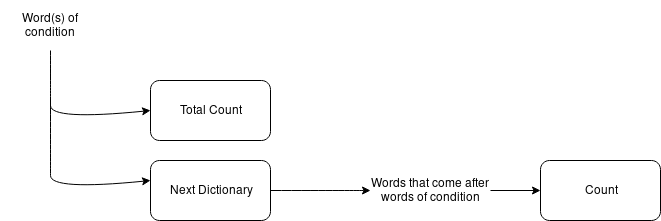
\includegraphics[width=1\linewidth, height=5cm]{asdf}

The structure above lets me to access data required in $O(1)$, while rescues me from the unnecessary memory usage like it would happen in a matrix.

Language Models follow the same equations for both essay generation and author detection, where n is equal to n-gram number:
\begin{gather}
n > 1: P(sentence) = \prod_{k=1}^mP(W_k | W_{k-1} W_{k-2} ... W_{k-n-1}) \\
n = 1: P(sentence) = \prod_{k=1}^mP(W_k)
\end{gather}

To avoid underflow and harder calculations, I work on a log space with these probabilities:
\begin{gather}
n > 1: P(sentence) = \sum_{k=1}^mlog(P(W_k | W_{k-1} W_{k-2} ... W_{k-n-1})) \\
n = 1: P(sentence) = \sum_{k=1}^mP(W_k)
\end{gather}

There may be also out of vocabulary words in test dataset. To avoid various errors I needed to use Laplace smoothing on probability calculations, such as the bi-gram equation below:

\begin{equation}
n = 2:
P(W | W_{k-1}) = \frac{C(W_{k-1}, W_k) + 1}{C(W_{k-1}) + V}
\end{equation}

where V is the number of the unique keys in models dictionary, namely condition words.
\subsection{Essay Generation}

In essay generation I forced my models to generate an essay with only 30 words maximum. Any tokens or punctuations aren't considered a word in the essays. I have used the next dictionary to quickly get the counts of next words after condition words in bi and tri-gram models. In uni-gram models I did not need to use the next dictionary at all since it is unnecessary to generate a essay with uni-gram.

The work-flow of generation is rather simple, an example with bi-gram is given below:
\begin{itemize}
\item[1.] Put one start token to beginning since n is 2.
\item[2.] Calculate the probabilities of the next words coming after the current word using equation 5.
\item[3.] Scale all of the probabilities to 1 and put them in an array.
\item[4.] Generate a random float between 0 and 1 and select the next word.
\item[5.] Repeat steps 2-4 until the end.
\end{itemize}

\begin{center}
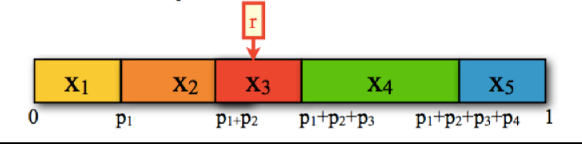
\includegraphics[width=0.7\linewidth, height=2cm]{essay}
\end{center}

\subsection{Author Detection}

In author detection the goal was to calculate the probability of the essays with both n-gram models using equations 3 or 4. Then the program picks the higher probability as the prediction of the author.
\section{Dataset}

There are some number of modifications to dataset in order to process it better. Firstly, I have filtered punctuations, except quotes, to have a white-space between the words around them. The main reason of that is I wanted to count them as separate tokens in my model. After that I put '\texttt{\_START\_}' and '\texttt{\_END\_}' tokens to start and end of all documents and also before and after every separated punctuation. Accordingly, by putting the end token my models actually learned which words end a sentence and which do not, so it can use a word, which was used before a comma, before a point to end a sentence. Similarly, with the start token my models can learn which words can start a sentence.

Furthermore, I have also reduced the number of words in the dictionary by shortening phrases like 'I am', 'You were not', ' He would not'. Accordingly, this helped me to reduce the complexity and get better results in both tasks. Additionally, all data is represented in lower-case except start and end tokens to again decrease the number of words in the dictionary.

\section{Results}

\bibliographystyle{IEEEtran}
\bibliography{references}

\end{document}
